\begin{figure}
\centering
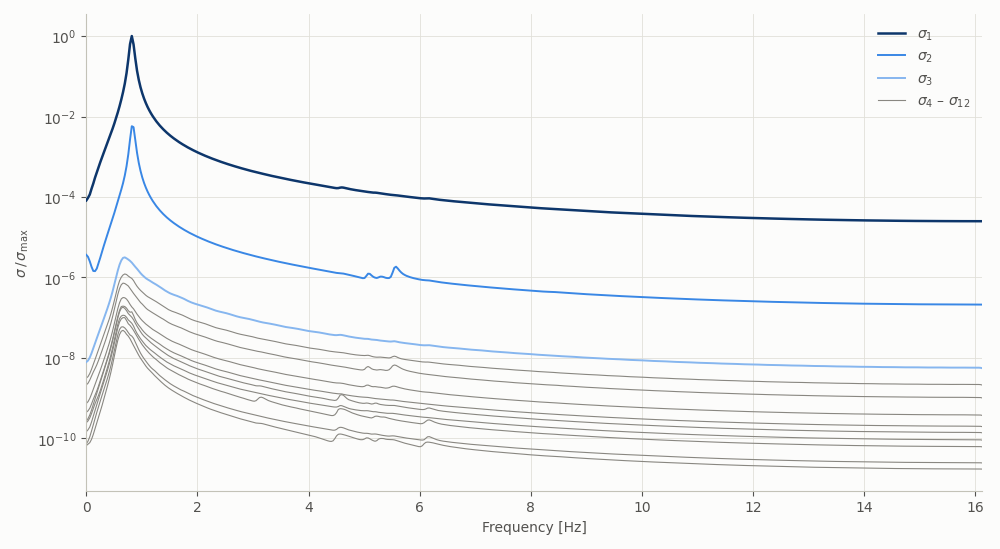
\includegraphics[width=\columnwidth]{figures/FDD-SV-plot-log.png}
\caption{
    MPE plot obtained from FSDD performed on a wind turbine. Note that the $y$-axis is plotted on a log-scale, which can help distinguish clustered modes from spurious peaks (noise). Measurements were collected from 4 accelerometers located at the base of the wind turbine tower, each measuring acceleration in three orthogonal directions. The plot shows an isolated peak in the largest SV around $0.8$, which is corroborated by a finite element model (FEM) of the tower that identified a natural frequency at $0.79$~\cite{PANDA2026124343}.
    }\label{fig:sv-plot}
\end{figure}